% !TEX root = morphkasten.tex

\section{Lagerung}


%##############
\subsection{Behälter}

\begin{figure} [hbp]
	\centering
	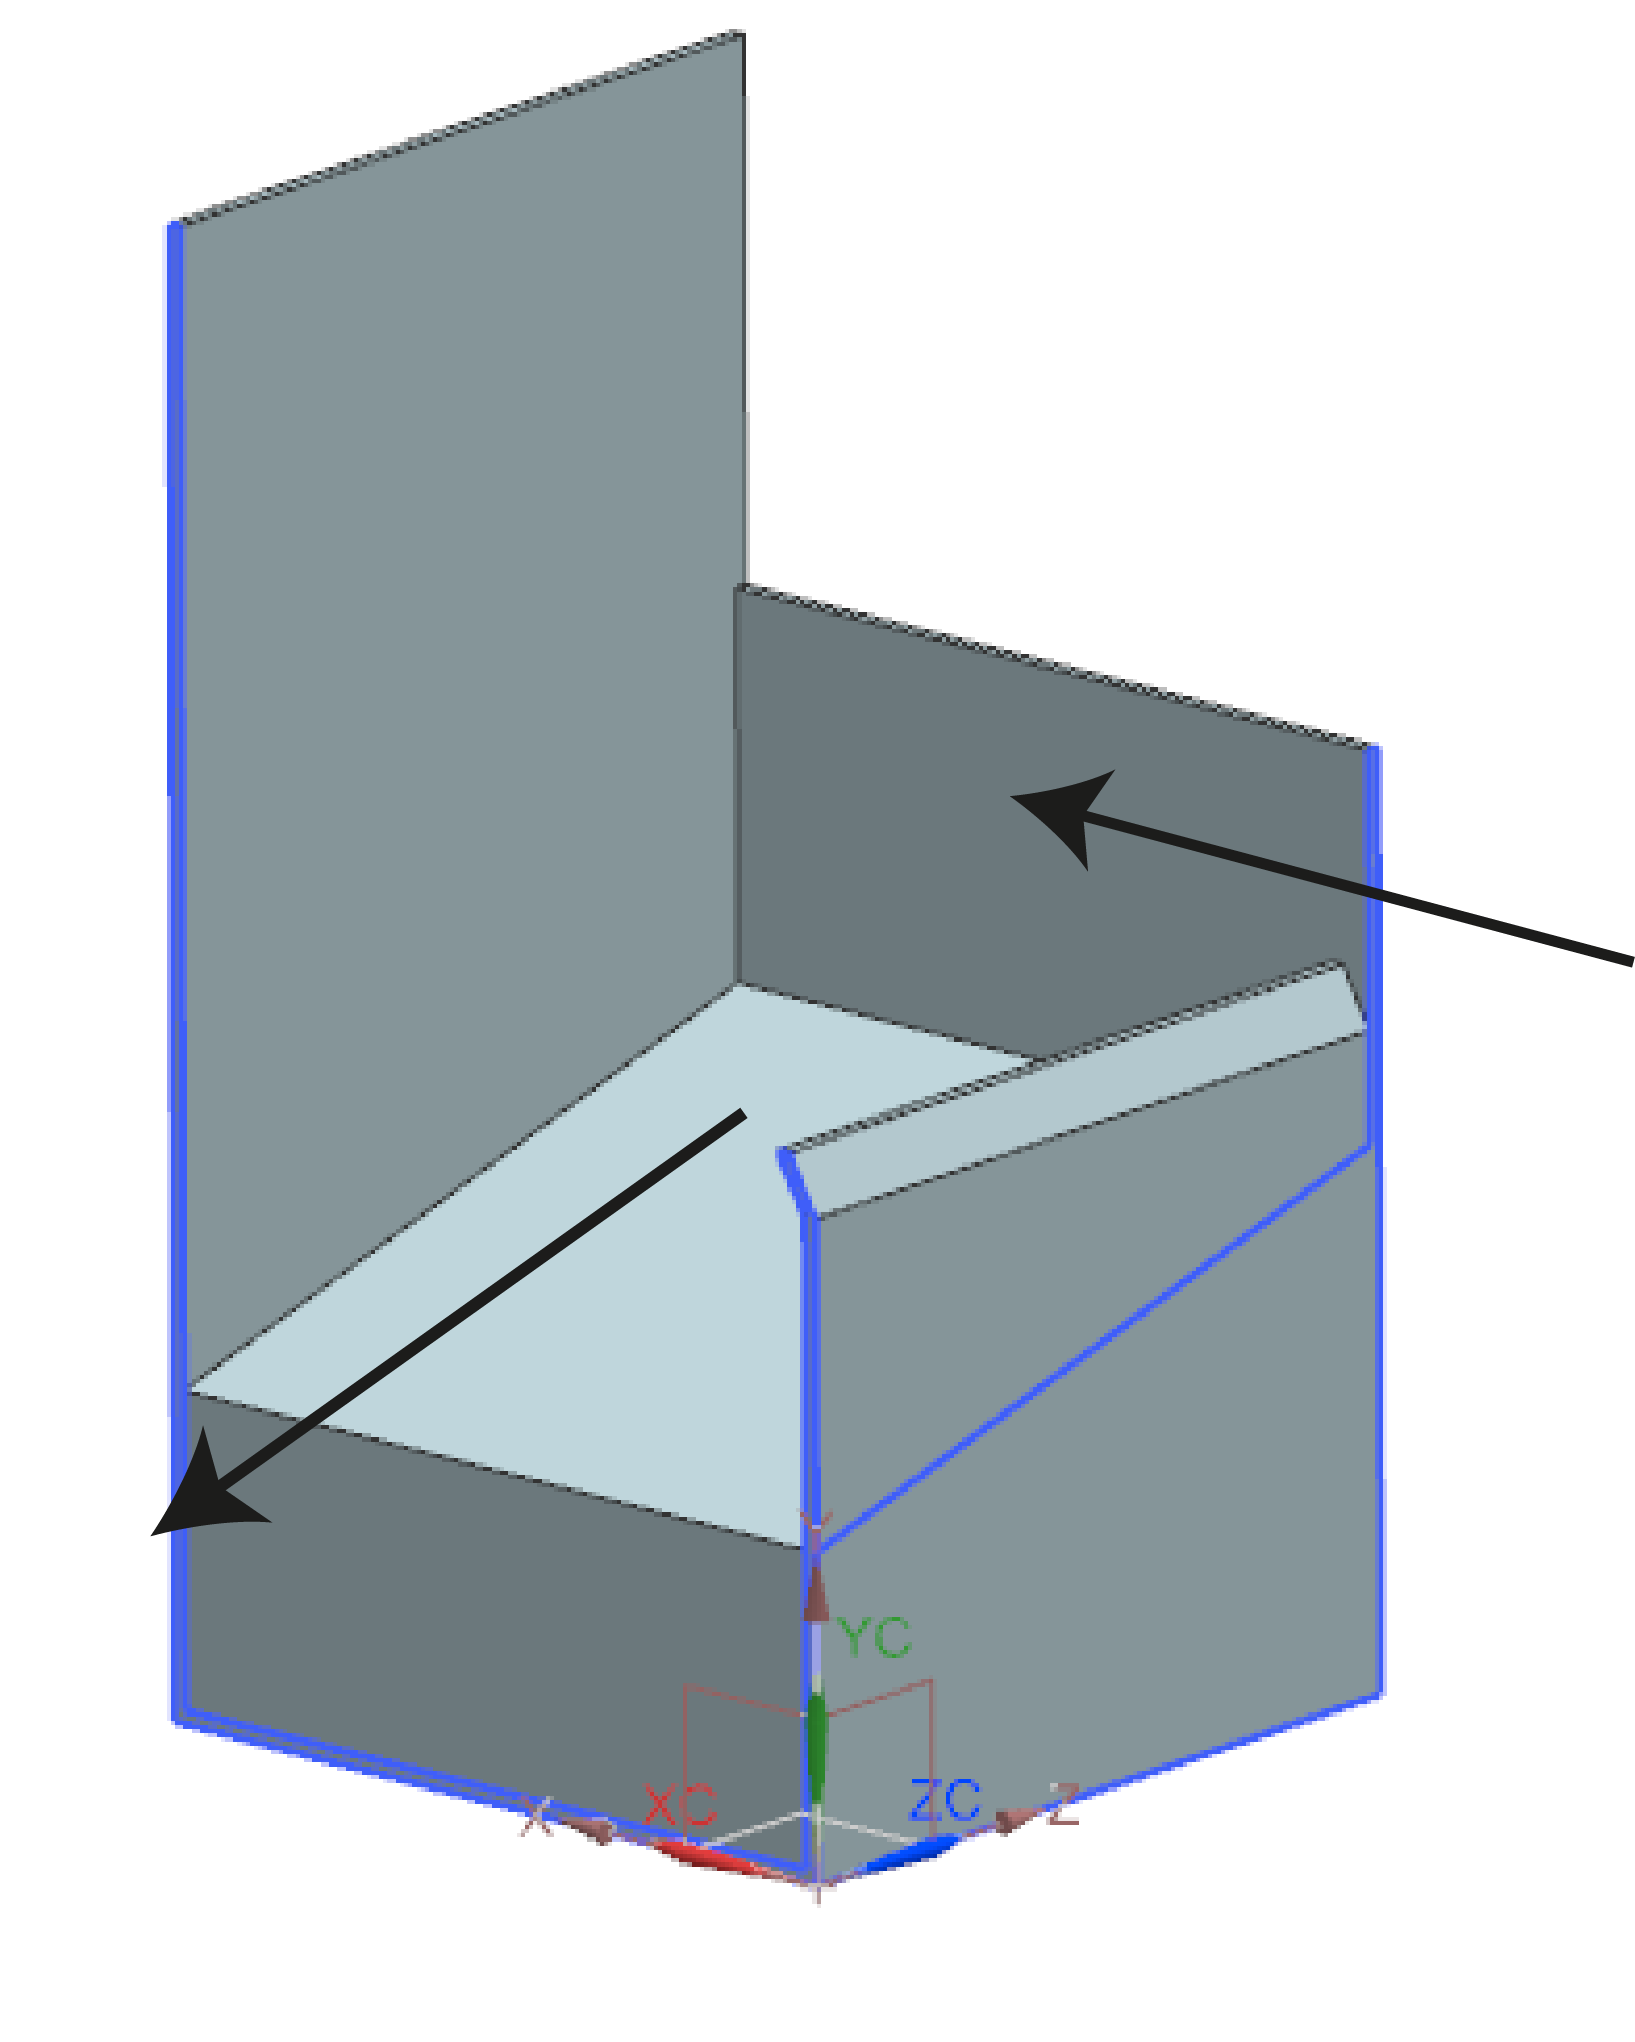
\includegraphics[width=0.3\textwidth]{fig/Unbenannt-1.png}
	\caption{Auffangbehälter, Schüttgutfluss mit Pfeilen angezeigt}
\end{figure}

\begin{table}[h]
\begin{tabular}{p{0.5\textwidth} | p{0.5\textwidth}}


 \textbf{Vorteile} & \textbf{Nachteile} \\ \hline
	 
\begin{itemize}
\item Keine elektrischen Komponenten notwendig
\item Vorgegebener Weg des Schüttguts
\end{itemize}

 
 &
 
\begin{itemize}
\item Maximale Höhe wird ausgenutzt
\item Aufwendiges Bauteil
\end{itemize}

\end{tabular}
\end{table}

\begin{table}[h]
\begin{tabular}{p{0.5\textwidth}p{0.5\textwidth}}


 \textbf{Risiken} & \\ \hline
	 
\begin{itemize}
\item Verschütten
\end{itemize}

 
\end{tabular}
\end{table}

\pagebreak
